\documentclass[a4paper, 11pt]{report}

    % preambule {{{
	\usepackage[utf8]{inputenc}
	\usepackage[T1]{fontenc}
    \usepackage[french]{babel}
	\usepackage[top=3cm,left=3cm,right=3cm,bottom=3cm]{geometry}
    \usepackage{lmodern}
    \usepackage{sectsty}
	\usepackage{graphicx}
    \usepackage{lastpage}
    \usepackage{fancyhdr}
    \pagestyle{fancy}
    \renewcommand{\headrulewidth}{0pt}
    \renewcommand{\footrulewidth}{.4pt}
    \lhead{}
    \chead{}
    \rhead{}
    \lfoot{\textsc{Lechat -- Wang -- Gaborit}}
    \cfoot{}
    \rfoot{\thepage/\pageref{LastPage}}

    \usepackage{fancyvrb} % pour forcer les verbatim sur une seule page
    \usepackage{url}

	\title{Comparaison de différents facteurs sur le procédé d'auralisation}
	\author{Thomas \textsc{Lechat} -- Xin \textsc{Wang} -- Mathieu \textsc{Gaborit} \hfill Encadrant : Christophe
    \textsc{Ayrault}}
	\date{L2 SPI
    \vskip 1cm
    Année universitaire 2012-2013}

	\makeatletter
	\def\thetitle{\@title}
	\def\theauthor{\@author}
	\def\thedate{\@date}
	\makeatother

    \sectionfont{
    \sectionrule{0pt}{0pt}{-5pt}{0.4pt}
    }

    % interligne
    \renewcommand{\baselinestretch}{1.1}

    \setcounter{secnumdepth}{5}
    \renewcommand{\thesection}{\Roman{section}.}
    \renewcommand{\thesubsection}{\Roman{section}.\Alph{subsection}.}
    \renewcommand{\thesubsubsection}{\arabic{subsubsection})}

    % }}}
    \newcommand\matlab{MATLab\textsuperscript{\textregistered}}
\begin{document}

% page de titre [PAS TOUCHE] {{{1
\begin{titlepage}

% logo Univ
\begin{flushright}

\includegraphics[width=4cm]{logo.png}
\end{flushright}


\vskip 6cm

% Titre
\begin{flushleft}
\huge{\textbf{Projet auralisation}}
\vskip .5cm
\hrule height 3pt
\vskip .5cm
\huge{\textbf{\thetitle}}
\end{flushleft}

\vfill

\begin{center}
\Large{
\thedate
}
\end{center}

\vskip 1cm
\hrule height .5pt
\vskip 1cm

\begin{flushleft}
\theauthor
\end{flushleft}

\end{titlepage}

% sommaire [PAS TOUCHE] {{{1
\renewcommand{\contentsname}{Sommaire
\vskip .5cm
\hrule height .5pt}
\tableofcontents
\newpage


% Chapitres {{{1
Pour le public, l'acoustique est un domaine s'appliquant principalement aux salles.
Bien que la majorité pense à l'amélioration des performances acoustiques, l'étude réelle autour des salles va
beaucoup plus loin.
La reproduction des conditions d'écoute dans une salle donnée (réelle ou virtuelle) est un sujet important. Il s'agit d'une
application à la frontière entre acoustique des salles et réalité virtuelle, le tout teinté de psychoacoustique. Dans les
domaines s'approchant, on citera notament la reproduction de transducteurs (en captation ou reproduction).

\medskip

Le fait de recréer la modification d'un son par une salle à partir de mesures ou de calculs s'appelle
l'\emph{auralisation}. L'auralisation est d'ailleurs définie ainsi dans l'ouvrage de Michael
Vorländer~\cit{vorlander2008} :

\begin{quote}
L'auralisation est une technique visant à créer des fichiers sonores écoutables depuis des données (simulées, mesurées
ou synthétisées) numériques.
\end{quote}

\medskip

Afin de mettre en œuvre une comparaison de l'influence de différents facteurs sur la qualité d'une auralisation, une
série de mesures est effectuée (réponses impulsionnelles -- RI --  binaurales et monaurales, sons en salles cibles,
etc...).  Ensuite, les signaux mesurés sont convolués avec les RI et le résultat est écouté et qualifié. Finalement, la
comparaison même prend forme et les résultats sont consignés et interprétés : il s'agit alors de comparer le résultat
obtenu par convolution «\emph{mathématique}» avec le rendu réel (convolution «\emph{physique}» en rejouant le son en
salle cible) et ce en variant divers paramètres (RI monaurale/binaurale, mode de convolution, etc...).

\chapter{Etat de l'art}

Les premiers essais se rapportant à l'auralisation ont été faits par Spandöck et coll. en 1929.
Ces travaux ont été repris et améliorés après l'apparition des ordinateurs ; en utilisant cette nouvelle puissance de
calcul et, vers la fin des années 1960, le premier logiciel de simulation d'acoustique des salles fut développé
(Krokstad)~\cite{Vor08}.

Le mot «auralisation» lui-même fut utilisé pour la première fois par Kleiner et coll. dans l'article
\underline{Auralization -- An Overview}~\cite{Kle93}.

Dans la sommes des techniques utilisées pour aboutir à la reproduction des conditions acoustiques d'une salle, deux
reviennent principalement :

\begin{itemize}
    \item utilsation de \item{ray-tracing} ;
    \item utilisation de systèmes source-image.
\end{itemize}

Les deux sont connues depuis longtemps et éprouvés, elles peuvent parallèlement être améliorer de la prise en compte de
divers facteurs :

\begin{itemize}
    \item diffusion (aléatoire ou déterminée)
    \item absorption
\end{itemize}

Les applications possibles de l'auralisation au terme général sont nombreuses et variées. La plus évidentes d'entre
elles est certainement la reproduction de «l'acoustique» d'une salle, mais on peut aller plus loin. L'acoustique
prédictive permet de simuler le rendu de salles et plus généralement d'espaces inexistants en combinant des mesures
entre elles ou purement par le calcul. Enfin, l'auralisation peut être utilisée dans la conception de systèmes de
réalité virtuelle à forte immersion.

Il faut enfin savoir que la complexité de rendu d'une auralisation rend difficile sa mise en place à grande échelle. Si
la projection en 3D et à 360 degrés est aujourd'hui possible \textit{via} divers processus de visualisation (le pendant
visuel de l'auralisation), l'inclusion d'un environnement acoustique pleinement contrôlé est extrèmement complexe et
demanderait un nombre impressionnant de haut parleurs (et ne pourrait s'adapter à chaque spectateur). Une restitution du
champ acoustique de manière individuelle peut être en revanche envisageable au travers de casques et d'un système de
suivi d'orientation 3D. Ce type d'environnement d'immersion existe soit en version prototypée (en Allemagne par exemple,
à Ilmenau) ou bien en version commerciale \textit{via} le projet
CAVE\textsuperscript{TM}\footnote{CAVE\textsuperscript{\textsc{TM}} :
    CAVE\textsuperscript{\textsc{TM}} Automatic Virtual
Environment}

\chapter{Principe de l'auralisation}

Le but de cette section est de mettre en lumière le procédé mathématique permettant l'auralisation d'une salle. Pour
cela nous allons nous intéresser à plusieurs notions qui rentrent en jeu dans l'auralisation.

\section{Produit de convolution} % {{{1
\label{produit_de_convo}

Ce projet traite uniquement de salles à taille réelle avec une source et un récepteur fixes. Dans ce cas particulier, la salle à étudier peut être assimilée à un filtre linéaire invariant par translation dans le temps. 

Pour qu'un système puisse être considéré comme linéaire, il suffit que pour des entrées $x_1(t)$ et $x_2(t)$ et leurs sorties respectives $y_1(t)$ et $y_2(t)$ on ait :
    
\begin{equation}
    \alpha x_1(t) + \gamma x_2(t) \Leftrightarrow \alpha y_1(t) + \gamma y_2(t)
\end{equation}

Dans notre cas, si 2 sons d'enveloppes et d'amplitudes différentes sont émis dans une salle, il parait logique ques ces sons n'interagiront pas entre eux et que par conséquent cette équation soit vérifiée dans le cas de l'émission d'un son dans une salle avec un émetteur et recépteur fixes.

On peut dire qu'un système est invariant par translation dans le temps si, alors qu'à un temps $t$ une entrée $x(t)$ est reliée à une sortie $y(t)$ on a pour un temps $t+\tau$ une entrée $x(t+\tau)$ liée à une sortie $y(t+\tau)$.

Dans le cadre de ce rapport, à la condition que ni l'émetteur ni le récepteur ne changent de position et que les conditions extérieures ne fluctuent pas trop (température, pression ambiante), la réponse d'une salle à un son donné n'a \textit{a priori} aucune raison de varier dans le temps.
Une salle peut donc bien être approximée à un système linéaire
On a donc le système présenté figure~\ref{systeme_lineaire_invariant}.

\begin{figure}[h!]
\begin{center}
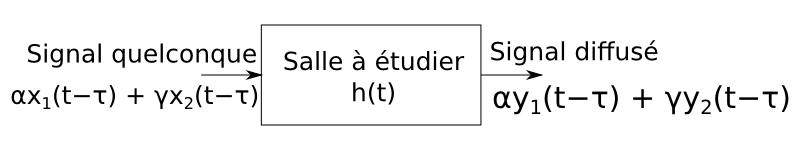
\includegraphics[width=10cm]{systeme_lineaire_invariant.png}
\end{center}
\caption{\label{systeme_lineaire_invariant}Le système à étudier est considéré invariant par translation dans le temps si
on peut lier les entrées aux sorties par une fonction de transfert constante pendant le temps considéré.}
\end{figure}


Comme les systèmes étudiés sont tous linéaires, il semble intéressant de  rappeler certaines des propriétés de ces systèmes.  
Sachant que le système est linéaire, on a donc :

\begin{equation}
    \alpha x_1(t) + \gamma x_2(t) \Leftrightarrow \alpha y_1(t) + \gamma y_2(t)
\end{equation}

Et

\begin{equation}     
    x_1(t)  \Leftrightarrow y_1(t)\\
    x_1(t -\tau) \Leftrightarrow y_1(t -\tau)                
\end{equation}

En combinant ces 2 propriétés on peut en déduire que :

\begin{equation}       
    \alpha x_1(t - \tau) + \gamma x_2(t - \tau) \Leftrightarrow \alpha y_1(t - \tau) + \gamma y_2(t - \tau)       
\end{equation}

On considère maintenant un signal quelconque $e(t)$. On peut approximer ce signal par une somme de signaux impulsionnels
$a_i(t)$ d'amplitudes différentes et décalés dans le temps (peigne de Dirac).
On a donc :

\begin{equation}        
    e(t) = \sum_{i} A_i a(t - \tau_i)
\end{equation}

Comme le système est linéaire on peut donc en déduire que la sortie du système s'écrira :

\begin{equation}        
    s(t) = \sum_{i} A_i h(t - \tau_i)
\end{equation}

Si on passe cette écriture à la limite continue~\cite{Mar12}, on obtient :

\begin{equation}        
    e(t) \to s(t) = \int e(\tau)h(t -\tau)d\tau
\end{equation}

Cette dernière relation est fondamentale et est nommée «produit de convolution». Ce produit est dénoté par le signe $\ast$.
De plus on constate que la fonction $h(t)$ correspond à la sortie du système pour une unique impulsion envoyée en entrée
(visible dans le cas ou on prend un $i$ unique).
Cette fonction est essentielle dans le processus d'auralisation, il s'agit de la fonction de tranfert caractérisant le système dans le domaine temporel, aussi nommée réponse impulsionnelle du système (RI).


\section{Mise en relation avec la transformée de Fourier} % {{{1

En termes de ressources et de temps de calcul, le produit de convolution est extrêmement lourd ; il est, de plus, peu maniable.
Il est toutefois possible de se servir d'une autre opération mathématique afin de rendre plus simple l'utilisation du produit de convolution.
La transformée de Fourier et l'espace de Fourier proposent des propriétés interessantes. Des algorithmes bien connus permettent de plus d'alléger le calcul et de l'accélérer (\textit{Fast Fourier Transform} notamment).
La transformée de Fourier est définie de la manière suivante:

\begin{equation}
    \mathcal{F}\{x(t)\} = \int_{-\infty}^{+\infty} x(t) e^{-2i\pi Ft} \mathrm dt
\end{equation}

Une des propriétés intéressantes concerne la transformée de Fourier d'un produit de convolution :

\begin{eqnarray*}
    \mathcal{F}\left\{x(t) \ast y(t)\right\} & = & \int_{-\infty}^{+\infty} \left[x(t) \ast y(t)\right] e^{-2i\pi Ft} \mathrm dt \\
    & = & \int_{-\infty}^{+\infty} \int_{-\infty}^{+\infty} x(u)y(t - \tau ) \mathrm du e^{-2i\pi Ft} \mathrm dt \\
    & = & \int_{-\infty}^{+\infty}  \left[ \int_{-\infty}^{+\infty} x(u)y(t - \tau )  e^{-2i\pi Ft} \right] \mathrm du \mathrm dt \\
\end{eqnarray*}

On pose $v= t- u$, on a donc $t= u+v$ à $u$ fixé,

\begin{eqnarray*}
    \mathcal{F}\left\{x(t) \ast y(t)\right\} & = & \int_{-\infty}^{+\infty}  \left[ \int_{-\infty}^{+\infty} x(u)y(v)  e^{-2i\pi F(v+u)} \right] \mathrm du \mathrm dv\\
    & = & \int_{-\infty}^{+\infty}  x(u) e^{-2i\pi Fu}  \mathrm du
    \int_{-\infty}^{+\infty} y(v) e^{-2i\pi Fv} \mathrm dv \\
    & = & \hat{x}(F) + \hat{y}(F)
\end{eqnarray*}

La transformée de Fourier du produit de convolution de 2 signaux est donc égale à la multiplication des transformées de Fourier de chacun des signaux.
Par conséquent, les calculs de produits de convolutions sont faits en passant par le domaine de Fourier pour
l'accélération des calculs (voir le paragraphe~\ref{acceleration_des_calculs}).


\section{Application à l'auralisation} % {{{1

Dans le cas d'un système linéaire on a :

\begin{equation}
e(t) \ast h(t) = s(t)
\end{equation}

Avec $e(t)$ le signal en entrée du système, $h(t)$ sa RI et $s(t)$ le signal en sortie du système pour $e(t)$ en entrée.
Dans le cas de l'auralisation d'une salle, le signal d'entrée correspond au signal anéchoïque à émettre dans la salle et le signal de sortie au signal enregistré une fois le système excité.
Lorsque la réponse impulsionnelle est connue (celle-ci étant facilement mesurable), il est possible, à partir de celle-ci et d'un son anéchoïque, d'en déduire le son tel qu'il pourrait être perçu si le signal anéchoïque avait été réellement émis dans la salle. C'est cette opération qu'on nomme auralisation.


Il faut cependant prendre en compte d'autres phénomènes dans le procédé d'auralisation, qui seront dûs au fait que notre source impulsionnelle excitatrice et la chaîne de mesure ne soient pas parfaites.
C'est lors de l'application des compensations pour les sources et chaîne de mesure que passer dans le domaine de Fourier
sera réellement utile pour limiter la complexité des calculs de convolution par simples multiplications et divisions de spectres.

\section{Essais Préliminaires}

Avant de chercher à comparer différentes techniques d'auralisation, une étude des moyens de comparaison et divers
essais préliminaires sont menés.

% TODO
%
% - comparaison entre RI recoupés et RI standard
% - nécessité du calage temporel
% - moyens de comparaison fréquentielle

\subsection{Fenêtrage temporel des réponses impulsionnelles} % {{{1

\begin{figure}[h!]
\centering{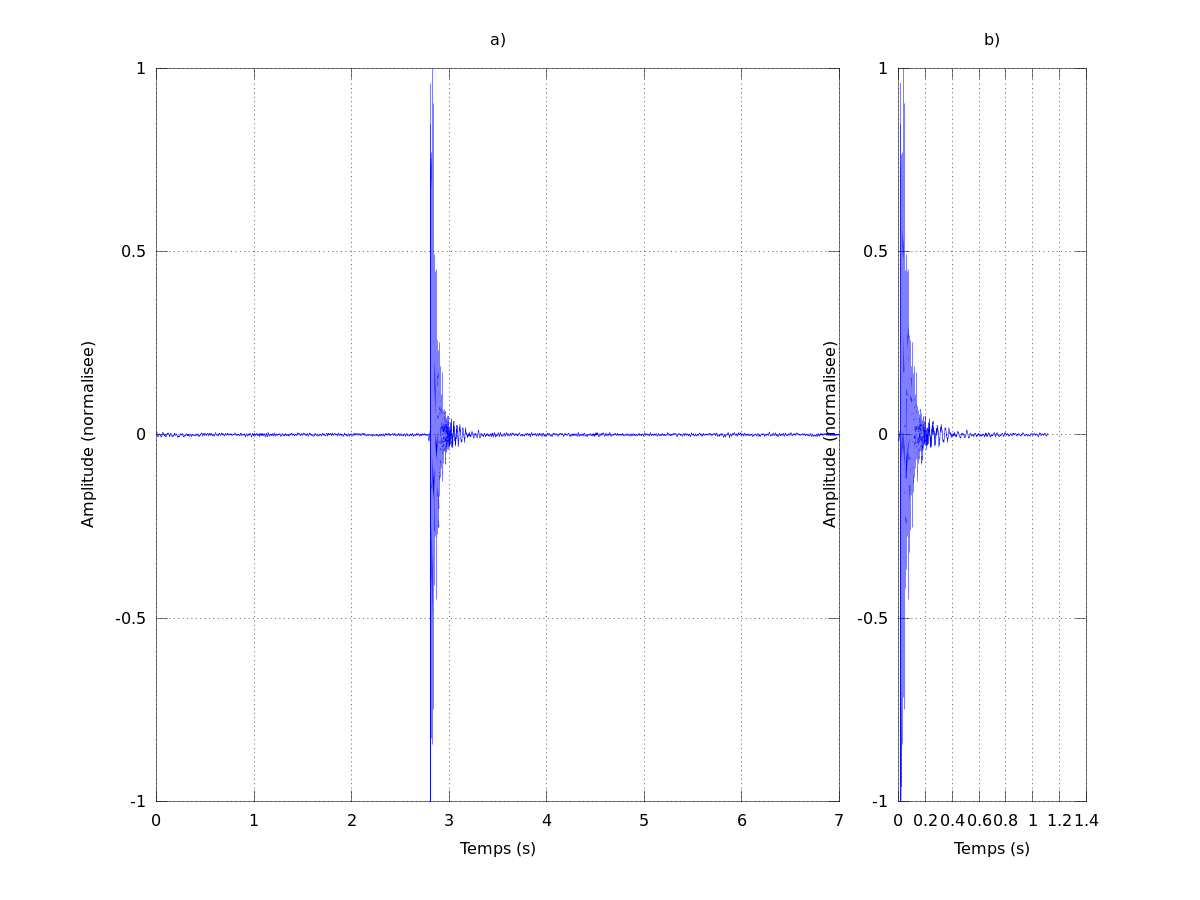
\includegraphics[width=15cm]{ri_non_recoupee.png}}
\caption{\label{ri_non_recoupee}Une des RI mesurées avant le fenêtrage (ici, le canal gauche d'une RI binaurale en salle
Mersenne). La figure a) montre la RI avant fenêtrage et la figure b) la même RI après fenêtrage}.
\end{figure}

Lors de la prise de réponses impulsionnelles, afin de ne pas dégrader l'information en «coupant» les réflexions les plus
tardives, les mesures sont faites sur des temps assez longs (voir figure~\ref{ri_non_recoupee});

De telles mesures posent plusieurs soucis, d'abord en terme de stockage mais aussi en terme de temps de calcul.

Les mesures de RI sont donc fenêtrées pour éliminer les blancs avant et après du traitement. Afin de conserver les
fichiers originaux et d'éviter l'apparition d'incohérences dans les fichiers de mesures, les fenêtrages sont codés en
dur dans les scripts de traitement et les fichiers de mesures sont laissés tels quels.

Il semble intéressant enfin de regarder quelle influence a le fenêtrage d'une RI sur le processus d'auralisation.

\begin{figure}[h!]
\centering{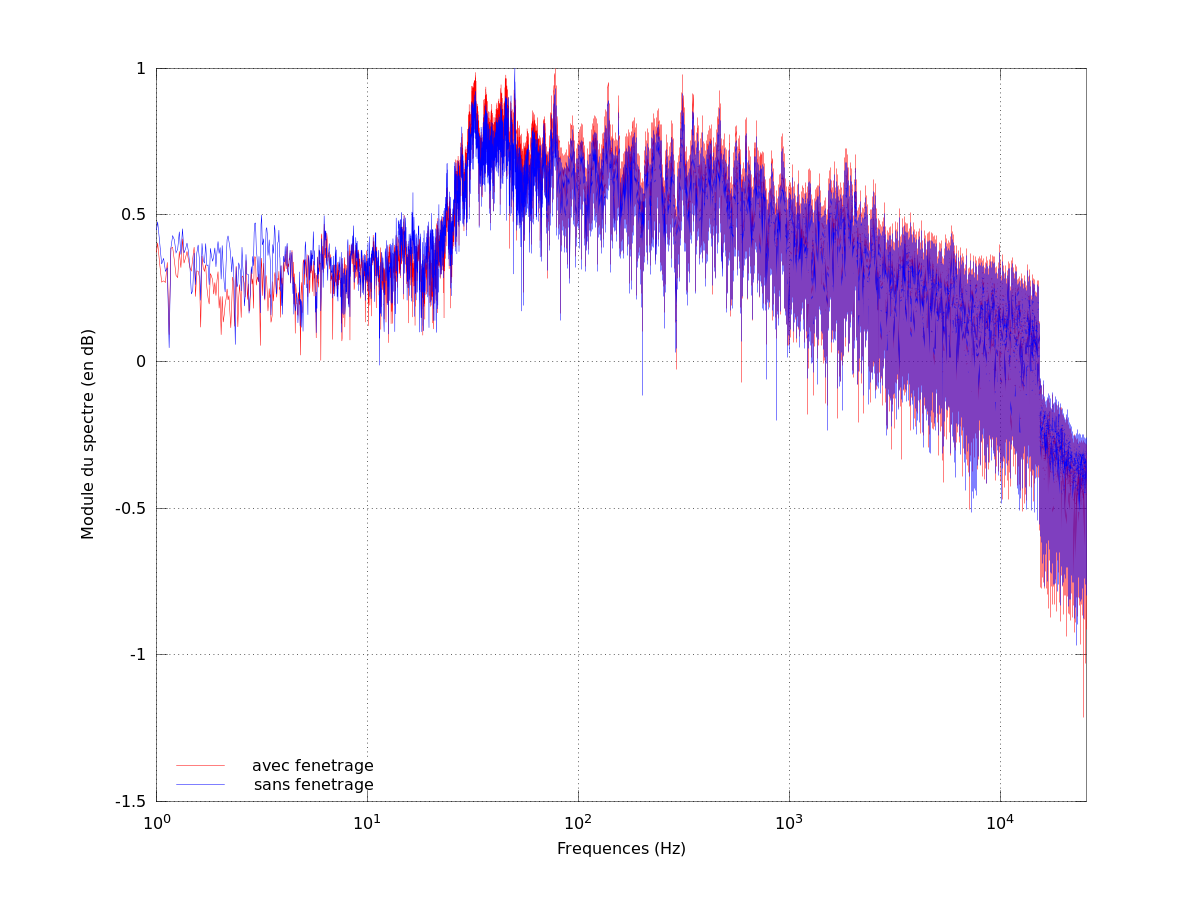
\includegraphics[width=15cm]{spks_ri_recoupe_superimposed.png}}
\caption{\label{spectres_recoupage}Les spectres des sons resultant de la convolution avec une RI fenêtrée (en rouge) et
non fenêtrée (en bleu). Même si les écarts sont faibles, ils existent.}
\end{figure}

Après deux tests, il apparaît que le fenêtrage des RI apporte un gain non négligeable en terme de temps de
calculs\footnote{une partie des calculs étant faits sur une machine peu puissante, cette composante est importante}.
Toutefois, comme le montre la figure~\ref{spectres_recoupage}, on remarque que les spectres de signaux convolués avec
une RI fenêtrée d'une part et non fenêtrés de l'autre ne sont pas identiques. Il faut malgré tout préciser que
perceptivement l'utilisation d'une RI fenêtrée rend le son plus net et moins bruité (plus réaliste en fait). Cela vient
probablement de l'élimination par fenêtrage du bruit de fond avant et après le son utile.

\subsection{Réduction du temps de calcul : procédé de convolution} % {{{1

La convolution est une opération mathématique très gourmande en temps processeur et en mémoire. Même si elle peut être
assez facilement parallèlisée\footnote{Soit avec des processeurs mathématiques dédiés soit avec des processeurs
hautement parallèles type GPU (processeurs de carte graphique)}, ces deux solutions étaient hors de portée ici.

La convolution joue dans le projet un rôle central puisqu'elle est l'outil permettant de passer d'une RI et d'un son
anéchoïque à un résultat sonore représentant la façon dont l'espace lié à la RI aurait modifié le son (voir
figure~\ref{lien_convo_projet}).

\begin{figure}[h!]
\centering{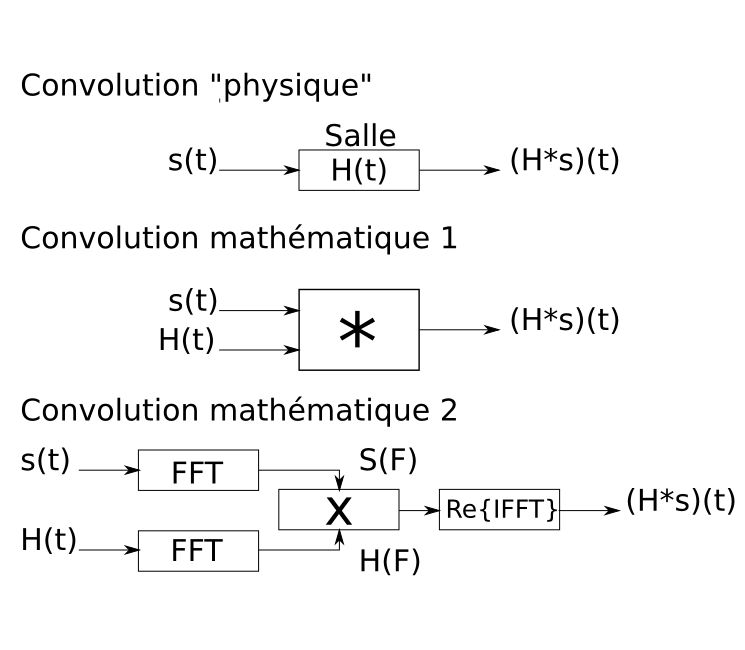
\includegraphics[width=9cm]{lien_convo_projet.png}}
\caption{\label{lien_convo_projet}Lien entre le projet et la convolution. En haut, la convolution «physique» (lorsque
qu'un signal $s(t)$ est émis dans la salle (de réponse impulsionnelle $H(t)$. Au milieu la convolution mathématique au
sens strict (\textit{via} l'opération consacrée). En bas, la convolution mathématique en utilisant la propriété de
symétrie entre convolution temporelle et multiplication fréquentielle. La chaine du bas est plus longue mais les calculs
sont plus rapides que pour celle du milieu.}
\end{figure}

La tranformée de Fourier (TF) est une opération qui n'est pas strictement réversible et qui entraine une légère perte de
données :

$$TF^{-1}\left\{TF\left\{s(t)\right\}\right\} \approx s(t)$$

La fonction \texttt{conv()} proposée par \matlab et GNU/Octave réalise une convolution mathématique stricte (au sens
discret). Celle ci est toutefois très lente sur des machines peu puissantes.

La fonction \texttt{fftconv()} proposée par GNU/Octave est par contre nettement plus rapide, elle utilise le mécanisme
présenté en bas de la figure~\ref{lien_convo_projet}. Cette fonction n'est toutefois pas proposée nativement dans
\matlab. Elle est réimplémentée pour le projet en s'appuyant sur un script trouvé sur le site utilisateurs du
logiciel\footnote{\url{http://www.mathworks.com/matlabcentral/fileexchange/5703-fftconv/content/fftconv.m}} :

\begin{Verbatim}[samepage=true]
function c = fftconv(a,b);

na = length(a);
nb = length(b);

n=na+nb;

A = fft(a,n);
B = fft(b,n);

c = ifft(A.*B,n);
c = real(c(1:na+nb-1));
\end{Verbatim}

Il semble intéressant de s'intéresser (au moins un peu) à l'erreur induite par l'utilisation de \texttt{fftconv()}
plutot que \texttt{conv}. La même convolution est réalisée avec chacune des fonctions, puis une simple distance
géométrique est utilisée pour calculer la distance existant entre les deux signaux : 

$$ d(t) = \sqrt{\left|\left[s_1(t)\right]^2 - \left[s_2(t)\right]^2\right|}$$

où $d(t)$ est la distance entre les signaux $s_1$ et $s_2$ au point d'abscisse $t$.

\begin{figure}[h!]
\centering{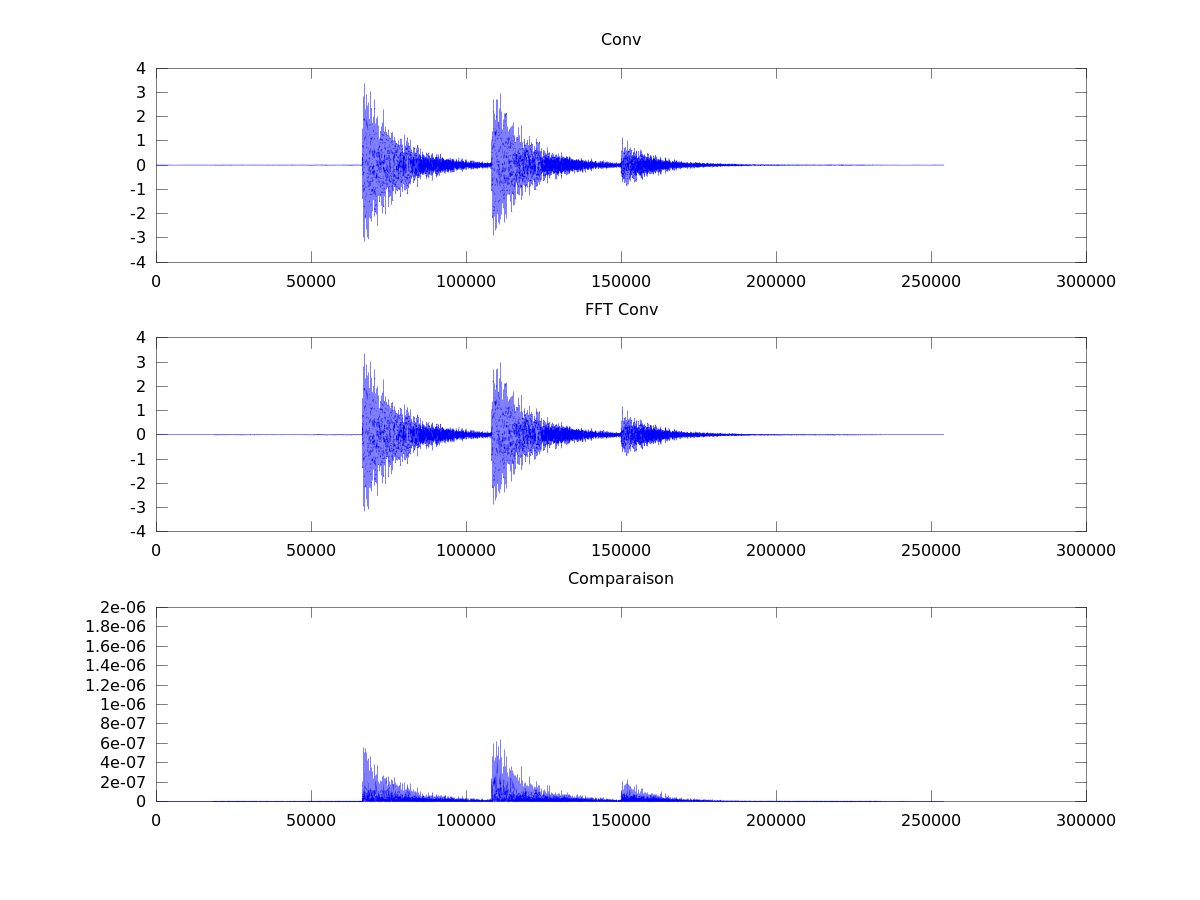
\includegraphics[width=12cm]{comp_conv_fftconv.png}}
\caption{\label{comp_conv_fftconv}Comparaison entre les résultats d'une même convolution avec \texttt{conv()} d'une part
et \texttt{fftconv()} d'autre part. On remarque notamment que sur le graphe du bas (représentant la distance géométrique
entre les 2 graphes au dessus), l'axe des ordonnées est gradué entre $2\cdot10^{-7}$ et $2\cdot10^{-6}$.}
\end{figure}

Le graphe obtenu est présenté en figure~\ref{comp_conv_fftconv}, il faut notamment noter que l'axe des ordonnées sur
le graphe des distances est gradué entre $2\cdot10^{-7}$ et $2\cdot10^{-6}$.

Devant la faible amplitude de l'erreur provoquée par l'utilisation de \texttt{fftconv()} et le gain en temps de calcul
réalisé, cette fonction semble largement plus avantageuse que \texttt{conv()}.

\subsection{Utlisation d'un ballon de baudruche} % {{{1

La réponse impulsionnelle d'une salle doit caractériser une salle et particulièrement les différentes réflexion induites
par sa géométrie.

Afin d'avoir une mesure la plus fidèle possible à la réalité du terrain, il faut que la source utilisée pour générer
l'impulsion (ou le bruit permettant la prise d'une réponse en fréquences) soit la plus omni-directionnelle possible.

L'utilisation d'un ballon de baudruche posait le souci que sa directivité est inconnue. Avec plus de temps, un
caractérisation de la directivité du ballon aurait pu être intéressante.

Une telle étude semble être en cours ou avoir été réalisée au LIMSI~\cite{Bru10}, malheureusement l'étude n'est pas
disponible à la consultation : pour ce projet, le ballon de baudruche sera donc considéré omnidirectionnel.

Le second incovénient soulevé par l'utilisation d'un ballon de baudruche est que la bande passante du son généré par
son éclatement n'est pas connu. Un éclatement de ballon de baudruche est donc mesuré en salle semi-anéchoïque (le
spectre est visible en figure~\ref{spk_ballon_anecho}.

\begin{figure}[h!]
\centering{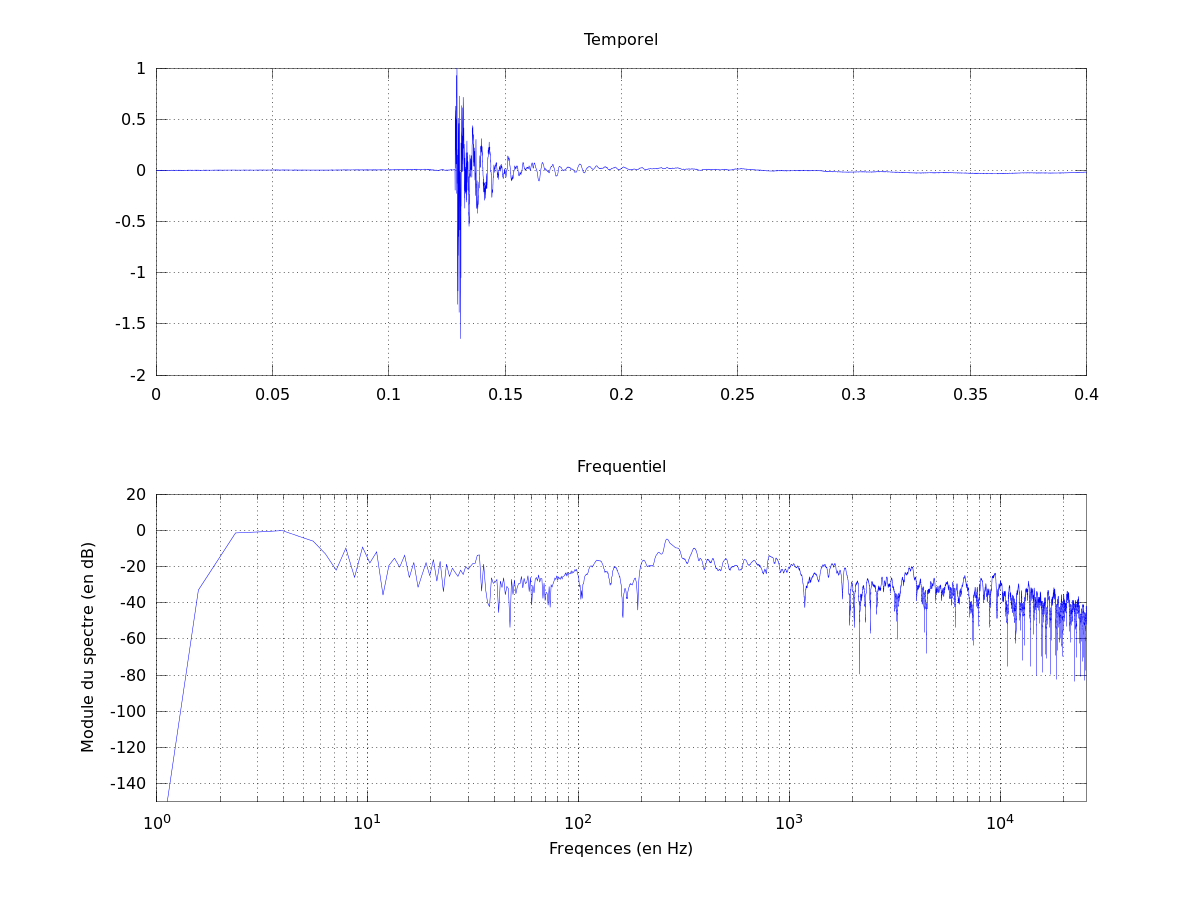
\includegraphics[width=15cm]{rep_ballon_anecho.png}}
\caption{\label{spk_ballon_anecho}}Enregistrement temporel de l'éclatement d'un ballon de baudruche en salle
semi-anéchoïque (noter la réflexions visible en temporel) et spectre du signal.}
\end{figure}

La réponse en fréquences n'est donc clairement pas plate. On note une décroissance de -20dB par décade et une série de
minima en hautes fréquences ainsi qu'un creux dans la bande 10 - 200Hz.

Une tentative de compensation des imperfections de la chaine d'excitation est décrite dans la suite.

\section{Comparaison monaural/binaural}

La perception sonore humaine est dite binaurale : c'est à dire qu'il y a deux «capteurs» (en l'occurence de chaque côté
de la tête).
Cette particularité est importante dans la perception de l'espace, en effet le volume de la tête retarde la propagation
du son tout en déformant celui-ci permettant ainsi un repérage dans le plan horizontal (avec une précsion pouvant aller
jusqu'a un degré~\cite{Vor08}). Le torse a lui aussi une influence, particulièrement pour le répérage dans le plan
vertical. Au cours des mesures pour ce projet, une tête artificielle (sans torse) a été utilisé, le repérage vertical
sera donc difficile à reproduire d'après nos mesures.



% }}}

% previous style : alpha
\bibliographystyle{alpha}
\bibliography{rapport}
\end{document}
